% Created 2020-04-24 vie 23:03
% Intended LaTeX compiler: pdflatex
\documentclass[12pt,a4paper, twoside]{article} % "twoside" en lugar de "twosite"
\usepackage[utf8]{inputenc}
\usepackage{pgf-umlcd}
\usepackage{lscape}
\usepackage{tikz}
\usepackage{tikz-qtree}
\usepackage{amssymb}
\usepackage{etoolbox}
\usepackage{xparse}
\usetikzlibrary{positioning, arrows.meta, shapes}
\usepackage[T1]{fontenc}
\usepackage{graphicx}
\usepackage{apalike}
\usepackage{xcolor}
\usepackage{multirow}
\usepackage{tabularx}
\usepackage{enumitem}
\usepackage{grffile}
\usepackage{longtable}
\usepackage{wrapfig}
\usepackage{rotating}
\usepackage[normalem]{ulem}
\usepackage{amsmath}
\usepackage{textcomp}
\usepackage{capt-of}
\usepackage[spanish]{babel}
\usepackage{grffile}
%\usepackage[dvips]{epsfig}
\usepackage{listings}
\let\bibhang\relax  % Elimina la definición previa de \bibhang
\usepackage[numbers]{natbib}
\usepackage{hyperref}
\usepackage[left=2.00cm, right=2.50cm, top=2.50cm, bottom=2.00cm]{geometry}
\usepackage{fancyhdr}
\fancyhead[RO,LE]{\thepage}
\fancyhead[LO]{\emph{\uppercase{\leftmark}}}
\fancyfoot{}
\renewcommand{\headrulewidth}{1.0pt}
\pagestyle{fancy}
\date{}
\title{Arquitectura de microprocesadores}
\hypersetup{
    pdfauthor={},
    pdftitle={Arquitectura de Microprocesadores},
    pdfkeywords={},
    pdfsubject={},
    pdfcreator={Emacs 26.2 (Org mode 9.1.9)},
    pdflang={ spanish }
}

\linespread{1.5}

\begin{document}

\renewcommand\refname{}
\renewcommand{\contentsname}{Tabla de contenido}
\newpage

\begin{titlepage}
    \begin{center}
        \vspace*{1cm}

                
\includegraphics[width=1\textwidth]{Figuras/logoFIUBA.pdf} % Ruta al logo de FIUBA

        \vspace{1.5cm}

        \textbf{\LARGE IP CORDIC modo rotador}

        \vspace{4cm}
        \textbf{\Large Arquitectura de microprocesadores}

        \vspace{1.5cm}


        \textbf{\Large Escrito por:}\\
        \large Karen Tatiana Zamudio

        \vspace{0.8cm}

        \textbf{\Large Revisión A}\\
        \large Nicolas Álvarez

        \vfill

        \textbf{\Large Universidad de Buenos Aires}\\
        \vspace{0.2cm}

        \large  11 junio 2024

    \end{center}
\end{titlepage}
\newpage

\section*{Historial de cambios}
\label{sec:registro}

\begin{table}[ht]
  \centering
  \caption{Registro de Revisiones}
  \label{tab:registro}
  \begin{tabularx}{\linewidth}{|c|X|c|}
    \hline
    Revisión & Detalles de los cambios realizados & Fecha \\
    \hline
    0 & Creación del documento & \ 01 de junio 2024 \\
    \hline
    1 & Entrega  & \ 11 de junio 2024 \\
    \hline
  \end{tabularx}
\end{table}

\maketitle
\tableofcontents

\newpage

\section{Introducción}
\label{sec:org60390fa}

El presente trabajo práctico final tiene como objetivo la implementación de un bloque de hardware digital en una FPGA, que formará parte de un sistema base de procesamiento junto con un micro Cortex A9.

Este bloque implementará un módulo de rotación basado en el algoritmo CORDIC (Coordinate Rotation Digital Computer) en modo rotador, el cual será una parte constitutiva del trabajo final de carrera del alumno. El funcionamiento del bloque incluirá la transferencia de datos entre el procesador y el módulo implementado, mediante un código C.


\subsection{Objetivos}
\label{subsec:org12e44a2}

Analizar y documentar el diseño, implementación y funcionamiento del módulo cordic rotator basado en el algoritmo CORDIC, así como evaluar su eficiencia y aplicabilidad en sistemas digitales.

\begin{enumerate}
    \item Implementar un módulo de rotación basado en el algoritmo CORDIC en Verilog.
    \item Simular todos los componentes del bloque principal.
    \item Sintetizar e implementar el diseño en una FPGA.
    \item Desarrollar una aplicación en C para la transferencia de datos entre el micro y el módulo de rotación CORDIC.
    \item Documentar el trabajo realizado, incluyendo una explicación del diseño, diagramas en bloques del circuito, capturas de simulaciones y tabla de uso de recursos de la FPGA.
    \item Configurar la FPGA y validar el funcionamiento del bloque implementado.
    \item Presentar los resultados en una presentación de 10 minutos en la última clase de la materia.
\end{enumerate}


\subsection{Alcance}
\label{subsec:org12e44a2}

El alcance de este trabajo final abarca la implementación y análisis de un módulo de rotación basado en el algoritmo CORDIC en una FPGA, como parte integral del trabajo final de carrera del alumno. Se llevará a cabo lo siguiente:

\begin{enumerate}

    \item Implementación del módulo de rotación CORDIC en VHDL/Verilog.
    \item Simulación exhaustiva del módulo para verificar su funcionamiento y precisión.
    \item Síntesis e implementación del diseño en una FPGA.
    \item Desarrollo de una aplicación en C para la transferencia de datos entre el micro y el módulo CORDIC.
    \item Documentación detallada del diseño, incluyendo explicaciones, diagramas en bloques, capturas de simulaciones y tabla de uso de recursos de la FPGA.
    \item Configuración y validación del funcionamiento del módulo implementado en la FPGA.
    \item Presentación de los resultados y análisis en una sesión de 10 minutos al finalizar la materia.
\end{enumerate}


El alcance de este trabajo final se centra en la implementación práctica del módulo de rotación CORDIC y su integración en un sistema de procesamiento basado en una FPGA. Se espera que este trabajo demuestre el dominio de los conceptos teóricos y prácticos adquiridos durante el curso, así como la capacidad para aplicarlos en un proyecto real.

\newpage

\section{CORDIC}
\label{sec:orgc1c4017}

CORDIC (Coordinate Rotation Digital Computer) es un algoritmo utilizado para calcular funciones trigonométricas, como seno, coseno, arcotangente, y para realizar rotaciones y transformaciones de coordenadas de manera eficiente en sistemas digitales. Fue desarrollado en la década de 1950 por Jack E. Volder en Bell Labs.

El algoritmo CORDIC se basa en una serie de rotaciones y desplazamientos sucesivos que permiten aproximar funciones trigonométricas y realizar operaciones de rotación con un bajo costo computacional. Una de las características clave del algoritmo CORDIC es su capacidad para realizar estas operaciones utilizando únicamente operaciones de suma, resta y desplazamiento bit a bit, lo que lo hace adecuado para implementaciones en hardware digital.

El algoritmo CORDIC es especialmente útil en aplicaciones donde se requieren cálculos trigonométricos rápidos y precisos, como en sistemas de procesamiento de señales, sistemas de comunicación digital, gráficos por computadora, entre otros. Además, es altamente versátil y puede adaptarse para calcular una amplia gama de funciones trigonométricas y realizar diversas operaciones geométricas.



\subsection{CORDIC trigonométrico}
\label{sec:orgdaca22c}


El algoritmo CORDIC (Coordinate Rotation Digital Computer) Trigonométrico es un método iterativo utilizado para calcular funciones trigonométricas como el seno ($\sin$), coseno ($\cos$), arcoseno ($\arcsin$) y arcocoseno ($\arccos$). Funciona mediante iteraciones de rotación y desplazamiento, donde cada iteración aproxima gradualmente el valor deseado de la función trigonométrica. El algoritmo se basa en la representación de un ángulo en coordenadas cartesianas $(X, Y)$ y utiliza rotaciones sucesivas para acercarse al ángulo objetivo. A medida que las iteraciones continúan, el valor de salida converge hacia el valor correcto con una precisión determinada.

En cada iteración del algoritmo CORDIC Trigonométrico, se realiza una rotación y un desplazamiento de las coordenadas $(X, Y)$. La rotación se realiza mediante el ajuste de los ángulos de las coordenadas, lo que permite acercarse al ángulo objetivo. El desplazamiento se utiliza para ajustar las magnitudes de las coordenadas y garantizar que la convergencia del algoritmo sea adecuada. Estas iteraciones se repiten hasta que se alcanza la precisión deseada en el cálculo de la función trigonométrica.

Por ejemplo, para calcular el seno de un ángulo dado utilizando el algoritmo CORDIC Trigonométrico, se inicializan las coordenadas $(X, Y)$ con valores apropiados y se realizan iteraciones de rotación y desplazamiento hasta que se alcanza la precisión deseada. El valor de $Y$ al final de las iteraciones representa el valor aproximado del seno del ángulo dado. De manera similar, se pueden calcular el coseno, el arcoseno y el arcocoseno utilizando adaptaciones del algoritmo CORDIC Trigonométrico.



La precisión y la convergencia del algoritmo CORDIC Trigonométrico dependen del número de iteraciones realizadas y del número de bits utilizados para representar los valores de las coordenadas. En general, el algoritmo converge rápidamente y proporciona resultados precisos con un número suficiente de iteraciones. Sin embargo, la precisión puede verse afectada por la representación finita de los números en sistemas digitales y por la resolución de las operaciones de rotación y desplazamiento.

El algoritmo CORDIC trigonométrico se utiliza en una amplia gama de aplicaciones en sistemas digitales, incluyendo procesamiento de señales, comunicaciones, gráficos por computadora, sistemas de navegación y más. Se utiliza para calcular funciones trigonométricas de manera eficiente y precisa en sistemas donde se requieren cálculos frecuentes de ángulos y funciones trigonométricas. Su implementación en hardware digital es especialmente adecuada debido a su simplicidad y eficiencia en términos de recursos computacionales.

Las ecuaciones para las iteraciones de rotación y desplazamiento en el algoritmo CORDIC Trigonométrico pueden ser expresadas como:

\begin{equation}
    \begin{aligned}
        X_{i+1} &= X_i - \delta_i \cdot Y_i \cdot 2^{-i}, \\
        Y_{i+1} &= Y_i + \delta_i \cdot X_i \cdot 2^{-i}, \\
        Z_{i+1} &= Z_i - \delta_i \cdot \text{atanh}(2^{-i}),
    \end{aligned}
\end{equation}

donde $i$ es el índice de iteración, $\delta_i$ es el signo de la rotación en la iteración $i$, $X_i$, $Y_i$ son las coordenadas en la iteración $i$, y $Z_i$ es el ángulo acumulado hasta la iteración $i$.  



\subsection{CORDIC vectorial}
\label{sec:orgdaca22c}


El algoritmo CORDIC Vectorial utiliza un enfoque similar al CORDIC Trigonométrico, pero se enfoca en manipular vectores en lugar de solo ángulos. Permite realizar rotaciones y transformaciones de coordenadas en sistemas de coordenadas cartesianas o polares de manera eficiente. 

En un sistema de coordenadas cartesianas, las operaciones del CORDIC Vectorial pueden utilizarse para rotar un vector en el plano XY. Por otro lado, en un sistema de coordenadas polares, el algoritmo puede utilizarse para convertir coordenadas cartesianas a polares y viceversa, así como para realizar rotaciones de vectores en el plano radial.

La eficiencia y precisión del CORDIC Vectorial lo hacen adecuado para una variedad de aplicaciones en sistemas digitales, como procesamiento de señales, modulación y demodulación en sistemas de comunicaciones, y transformaciones geométricas en gráficos por computadora. Además, su estructura iterativa permite su implementación eficiente en hardware digital, lo que lo convierte en una opción popular en sistemas embebidos y sistemas de tiempo real donde los recursos son limitados.


\subsection{CORDIC logarítmico}
\label{sec:orgdaca22c}

El algoritmo CORDIC logarítmico utiliza una serie de iteraciones para aproximar funciones logarítmicas y exponenciales, así como operaciones relacionadas como la raíz cuadrada y el exponente. A través de un proceso iterativo, el algoritmo calcula las aproximaciones de estas funciones con una precisión deseada.

Una de las características clave del CORDIC logarítmico es su capacidad para calcular estas funciones de manera eficiente y precisa utilizando un enfoque iterativo y estructuras de datos simples. Esto lo hace adecuado para su implementación en sistemas digitales donde se requieren cálculos de funciones no trigonométricas con recursos limitados.

El CORDIC logarítmico tiene una amplia gama de aplicaciones en sistemas digitales, incluyendo procesamiento de señales, compresión de datos, criptografía y más. Se utiliza en situaciones donde se requiere el cálculo rápido y preciso de funciones logarítmicas y exponenciales, así como operaciones relacionadas como la raíz cuadrada y el exponente. Su eficiencia y precisión lo hacen valioso en una variedad de aplicaciones de sistemas digitales.


\newpage

\section{Descripción del módulo CORDIC modo rotador}
\label{sec:descripcion}

En esta sección, se detalla la implementación del módulo CORDIC Rotator en Verilog. El módulo CORDIC Rotator es una implementación hardware del algoritmo CORDIC (Coordinate Rotation Digital Computer), diseñado para realizar rotaciones de vectores en el plano cartesiano. El algoritmo CORDIC se utiliza ampliamente en sistemas digitales para calcular funciones trigonométricas, transformaciones de coordenadas y otras operaciones matemáticas de manera eficiente. A continuación, se explicará paso a paso la implementación del módulo CORDIC rotator, incluyendo la configuración de parámetros, la definición de la tabla de arco tangente, las iteraciones del algoritmo y la salida del módulo. Cada parte de la implementación se analizará en detalle, acompañada de su correspondiente código en Verilog.

Para comenzar, el código inicia con la configuración del \texttt{timescale} y la definición de parámetros utilizados en el módulo. El parámetro \texttt{c\_parameter} determina el ancho de bits de los datos de entrada y salida, mientras que \texttt{STG} se utiliza para definir el ancho de bits de los vectores \texttt{X} e \texttt{Y}. Luego, se declara el módulo \texttt{cordic\_rotator} con sus entradas (\texttt{clock}, \texttt{angle}, \texttt{Xin}, \texttt{Yin}) y salidas (\texttt{Xout}, \texttt{Yout}).

\begin{lstlisting}[language=Verilog]
`timescale 1ns/100ps

module cordic_rotator (
    input clock,
    input signed [31:0] angle,
    input signed [c_parameter - 1:0] Xin,
    input signed [c_parameter - 1:0] Yin,
    output signed [c_parameter:0] Xout,
    output signed [c_parameter:0] Yout
);

parameter c_parameter = 16;
localparam STG = c_parameter;
\end{lstlisting}

La tabla \texttt{atan\_table} contiene los valores de la función arco tangente utilizados en el algoritmo CORDIC. Estos valores están precalculados y se utilizan para realizar las operaciones de rotación en el módulo. La tabla está definida como un arreglo de 31 bits con 31 entradas, cada una representando un ángulo específico.

\begin{lstlisting}[language=Verilog]
wire signed [31:0] atan_table [0:30];
assign atan_table[00] = 32'b00100000000000000000000000000000; 
// Resto de asignaciones de la tabla atan_table...
\end{lstlisting}

Se inicializan los registros \texttt{X}, \texttt{Y} y \texttt{Z}, que se utilizan para almacenar los datos en cada etapa del algoritmo CORDIC. Luego, se calcula el cuadrante en el que se encuentra el ángulo de rotación para determinar cómo se deben tratar los datos de entrada.

\subsection{Cuadrante I}

En el cuadrante I, el ángulo de rotación se encuentra en el rango de 0 a $\pi$/2. En este caso, no es necesario realizar ninguna modificación en los datos de entrada, ya que están en el rango adecuado para ser procesados por el algoritmo CORDIC. Por lo tanto, los valores de las coordenadas X e Y del vector de entrada (\texttt{Xin} y \texttt{Yin}) se asignan directamente a los registros \texttt{X[0]} y \texttt{Y[0]}, respectivamente. Además, el ángulo de rotación (\texttt{angle}) se asigna directamente al registro \texttt{Z[0]}.

\begin{lstlisting}[language=Verilog]
       case (quadrant)
           2'b00: begin // Cuadrante I
               X[0] <=   Xin;
               Y[0] <=   Yin;
               Z[0] <=   angle;
\end{lstlisting}

Este caso se activa cuando los bits de signo del ángulo son 0, indicando que el ángulo se encuentra en el primer cuadrante.

\subsection{Cuadrante II}

En el cuadrante II, el ángulo de rotación se encuentra en el rango de $\pi$/2 a $\pi$. Para ajustar los datos de entrada al rango adecuado para el algoritmo CORDIC, se realiza una pre-rotación del ángulo. En este caso, el ángulo se resta de $\pi$ para asegurar que esté dentro del rango de -$\pi$/2 a 0. Los valores de las coordenadas X e Y del vector de entrada se asignan a los registros \texttt{X[0]} y \texttt{Y[0]}, respectivamente, de la misma manera que en el cuadrante I.

\begin{lstlisting}[language=Verilog]
       2'b01: begin // Cuadrante II
               X[0] <=    Xin;
               Y[0] <=    Yin;
               Z[0] <=  32'b10000000000000000000000000000000 - angle;                  
\end{lstlisting}

Este caso se activa cuando el bit de signo más significativo del ángulo es 0 y el siguiente bit es 1, indicando que el ángulo se encuentra en el segundo cuadrante.

\subsection{Cuadrante III}

En el cuadrante III, el ángulo de rotación se encuentra en el rango de -$\pi$ a -$\pi$/2. Al igual que en el cuadrante II, se realiza una pre-rotación del ángulo restando $\pi$ para asegurar que esté dentro del rango de -$\pi$/2 a 0. Los valores de las coordenadas X e Y del vector de entrada se asignan a los registros \texttt{X[0]} y \texttt{Y[0]}, respectivamente, de la misma manera que en los cuadrantes I y II.

\begin{lstlisting}[language=Verilog]
       2'b10: begin // Cuadrante III
               X[0] <=    Xin;
               Y[0] <=    Yin;
               Z[0] <=    angle - 32'b10000000000000000000000000000000; 
\end{lstlisting}

Este caso se activa cuando el bit de signo más significativo del ángulo es 1 y el siguiente bit es 0, indicando que el ángulo se encuentra en el tercer cuadrante.

\subsection{Cuadrante IV}

En el cuadrante IV, el ángulo de rotación se encuentra en el rango de -$\pi$/2 a 0. Para ajustar los datos de entrada al rango adecuado para el algoritmo CORDIC, se realiza una pre-rotación del ángulo restando 2$\pi$ para asegurar que esté dentro del rango de -$\pi$/2 a -$\pi$. Los valores de las coordenadas X e Y del vector de entrada se asignan a los registros \texttt{X[0]} y \texttt{Y[0]}, respectivamente, de la misma manera que en los cuadrantes I, II y III.

\begin{lstlisting}[language=Verilog]
       2'b11: begin // Cuadrante IV
               X[0] <=    Xin;
               Y[0] <=    Yin;
               Z[0] <=    angle - 32'b10000000000000000000000000000000; 
\end{lstlisting}

Este caso se activa cuando los bits de signo del ángulo son 1, indicando que el ángulo se encuentra en el cuarto cuadrante.

\newpage

\section{Creación de la IP}

Para crear una IP personalizada que incluya el módulo \texttt{cordic\_rotator}, se puede utilizar el template de periférico esclavo de Vivado. A continuación se describen los pasos para realizar esta tarea.

\subsection{Usar el template de periférico esclavo}

Para comenzar, abre Vivado seleccionando \textit{Start $\rightarrow$ Xilinx Design Tools $\rightarrow$ Vivado 2018.1}. Luego, haz clic en \textit{Manage IP}, elige \textit{New IP Location}, y selecciona \textit{Next} en la ventana \textit{New IP Location}. Selecciona la placa correspondiente, \textit{verilog} como \textit{Target Language}, y \textit{Mixed} como \textit{Simulator Language}. Para el campo \textit{IP Location}, elige una ubicación como, por ejemplo, el lugar donde se encuentran todas las prácticas y crea una carpeta \textit{cordic\textunderscore ip}. Presiona \textit{Finish}. Si el directorio no existe, se solicitará la creación.

\subsection{Integración del Módulo}


Para integrar el módulo \texttt{cordic\_rotator} con \texttt{Cordic\_ip\_v1\_0\_S\_AXI}, se deben tener en cuenta varios parámetros y registros. Los parámetros importantes incluyen el ancho del bus de datos AXI (\textbf{C\_S\_AXI\_DATA\_WIDTH}) que se configura en 32 bits, y el ancho del bus de direcciones AXI (\textbf{C\_S\_AXI\_ADDR\_WIDTH}) que se configura en 5 bits. Además, el ancho de bits para las entradas y salidas del módulo CORDIC (\textbf{c\_parameter}) se configura en 16 bits.

\begin{figure}[ht]
\centering
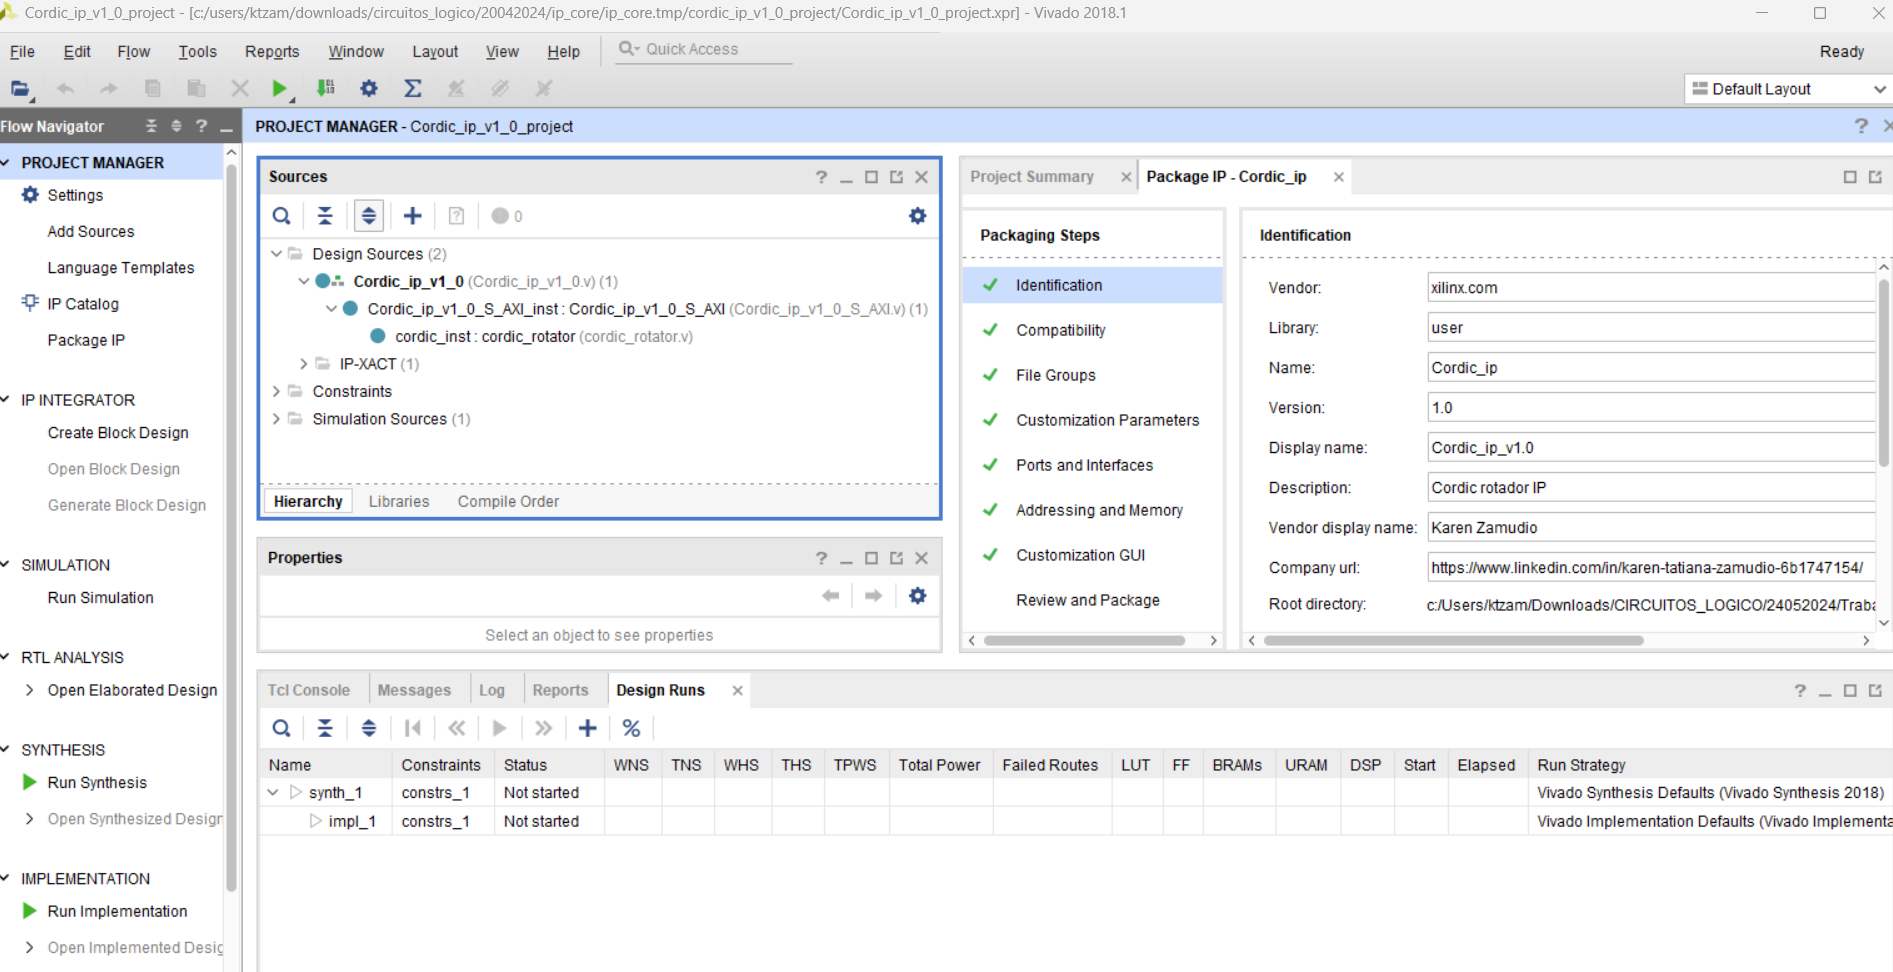
\includegraphics[width=0.8\textwidth]{./Figuras/sources_ip.png}
\captionof{figure}{Integración de modulos IP.}
\label{fig:Integración de modulos IP}
\end{figure}


Los registros de usuario (\texttt{slv\_reg0} a \texttt{slv\_reg4}) almacenan los datos que se enviarán al módulo \texttt{cordic\_rotator} y recibirán los resultados de este. \texttt{slv\_reg0} contiene el ángulo de rotación (32 bits), \texttt{slv\_reg1} almacena el valor de entrada X (16 bits), y \texttt{slv\_reg2} el valor de entrada Y (16 bits). Las salidas del módulo CORDIC, \texttt{Xout} y \texttt{Yout}, se almacenan en \texttt{slv\_reg3} y \texttt{slv\_reg4} respectivamente, ambas de 17 bits.

El módulo \texttt{cordic\_rotator} tiene varias señales importantes que permiten su funcionamiento correcto. Entre las entradas se encuentran la señal de reloj (\texttt{clock}), que sincroniza las operaciones del módulo, y la señal de ángulo de rotación (\texttt{angle}), que define el ángulo en el que se realizará la rotación CORDIC. Además, el módulo recibe dos valores de entrada, X (\texttt{Xin}) y Y (\texttt{Yin}), que son las coordenadas del punto que se desea rotar. Estas señales de entrada son cruciales para que el módulo pueda calcular las nuevas coordenadas del punto después de aplicar la rotación. Las salidas del módulo son los valores rotados (\texttt{Xout} y \texttt{Yout}), que representan las nuevas coordenadas del punto rotado. Estas salidas se obtienen después de que el módulo procesa las entradas a través del algoritmo CORDIC. A continuación se muestra un diagrama que ilustra la conexión entre los módulos:


\begin{figure}[ht]
\centering
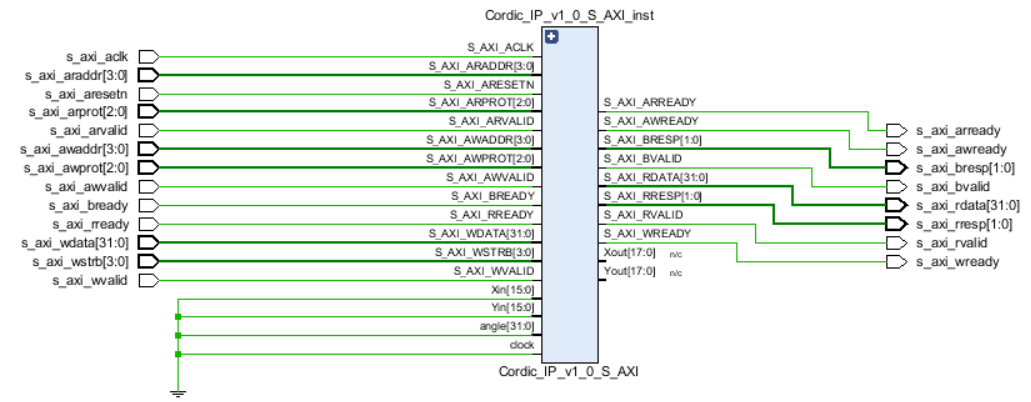
\includegraphics[width=0.8\textwidth]{./Figuras/arquitectura_de_ip_sin_maximizar.png}
\captionof{figure}{Diagrama de conexión del módulo minimizado \texttt{cordic\_rotator} con \texttt{Cordic\_ip\_v1\_0\_S\_AXI}.}
\label{fig:Diagrama de conexión del módulo minimizado}
\end{figure}
   

La asociación entre \texttt{Cordic\_ip\_v1\_0\_S\_AXI} y \texttt{cordic\_rotator} se realiza conectando las señales de entrada y salida del módulo \texttt{cordic\_rotator} a los registros adecuados del módulo \texttt{Cordic\_ip\_v1\_0\_S\_AXI}. La conexión se realiza como sigue:

\begin{verbatim}
cordic_rotator cordic_inst (
    .clock(S_AXI_ACLK),
    .angle(slv_reg0),
    .Xin(slv_reg1),
    .Yin(slv_reg2),
    .Xout(Xout),
    .Yout(Yout)
);
\end{verbatim}

El proceso de escritura y lectura de datos en los registros se maneja a través de la interfaz AXI. Cuando se recibe una dirección y datos válidos, estos se escriben en los registros correspondientes. Los valores de entrada y el ángulo se transfieren a \texttt{slv\_reg0}, \texttt{slv\_reg1} y \texttt{slv\_reg2}, respectivamente.

\begin{figure}[ht]
\centering
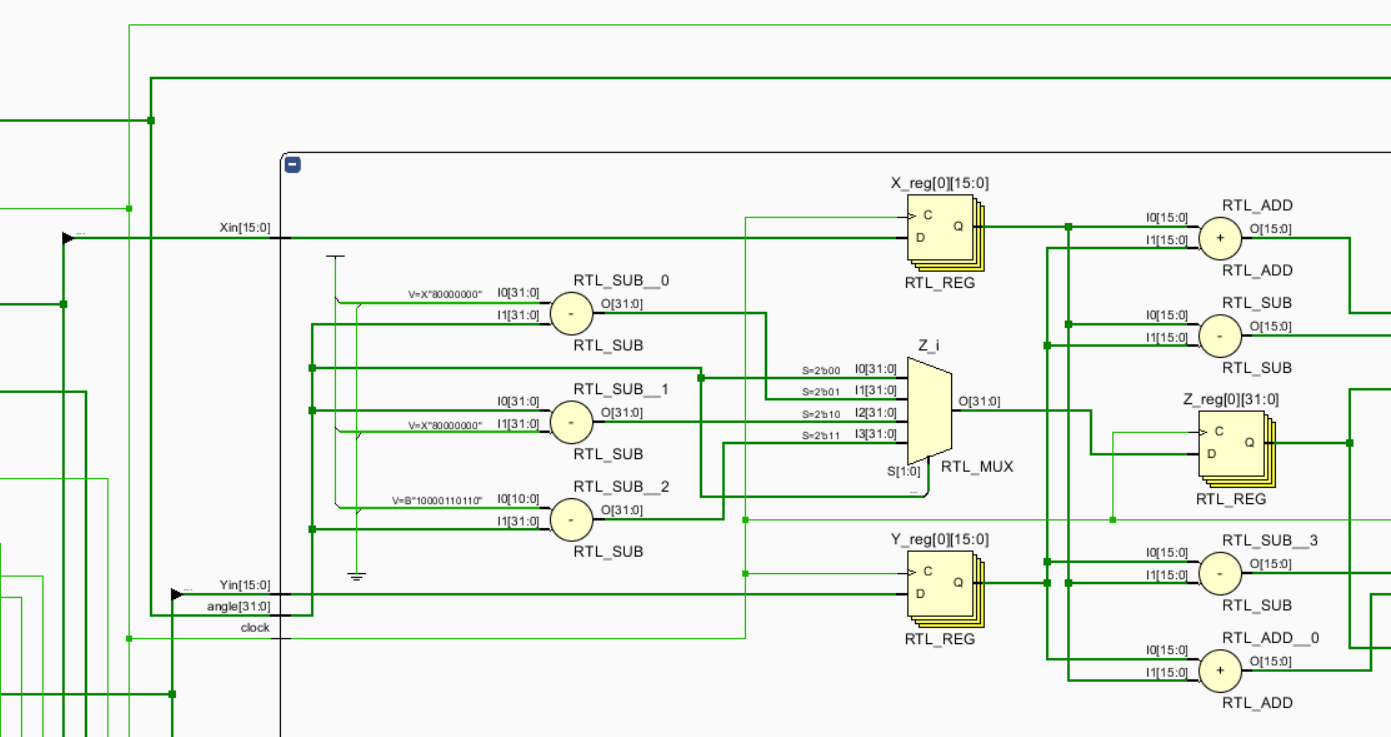
\includegraphics[width=0.8\textwidth]{./Figuras/entradas_cordic.png}
\captionof{figure}{Diagrama de conexión del módulo (entradas) \texttt{cordic\_rotator} con \texttt{Cordic\_ip\_v1\_0\_S\_AXI}.}
\label{fig:Diagrama de conexión del módulo minimizado}
\end{figure}

El módulo \texttt{cordic\_rotator} procesa estos datos para realizar la rotación CORDIC y los resultados se almacenan en \texttt{Xout} y \texttt{Yout}. Finalmente, los resultados de la rotación se leen a través de la interfaz AXI desde \texttt{slv\_reg3} y \texttt{slv\_reg4}.

\begin{figure}[ht]
\centering
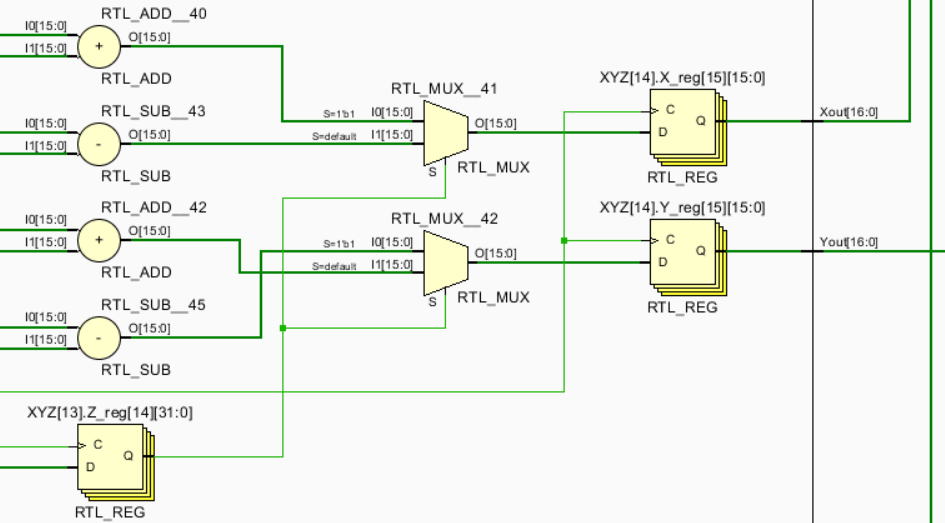
\includegraphics[width=0.8\textwidth]{./Figuras/salidas_ip.png}
\captionof{figure}{Diagrama de conexión del módulo (salidas) \texttt{cordic\_rotator} con \texttt{Cordic\_ip\_v1\_0\_S\_AXI}.}
\label{fig:Diagrama de conexión del módulo minimizado}
\end{figure}




\subsection{Descripción del flujo de trabajo creación IP en vivado}

El flujo de trabajo de implementación de IP en Vivado Design Suite sigue una serie de etapas bien definidas para garantizar el desarrollo efectivo y la integración de los bloques de propiedad intelectual. Comienza con la creación del IP, donde se desarrolla el código fuente junto con la documentación y los archivos de prueba necesarios. Luego, el IP se empaqueta en un archivo que incluye toda la información relevante para su uso en otros diseños, lo que implica configuración, simulación y generación de documentación. A continuación, se lleva a cabo una fase de simulación para verificar la funcionalidad y detectar posibles errores, seguida de un análisis RTL para identificar problemas de diseño. Una vez completadas estas etapas, el código fuente se sintetiza en una representación de circuito lógico y se implementa en el dispositivo FPGA de destino, optimizando la colocación y la ruta de las celdas lógicas.


\begin{figure}[ht]
\centering
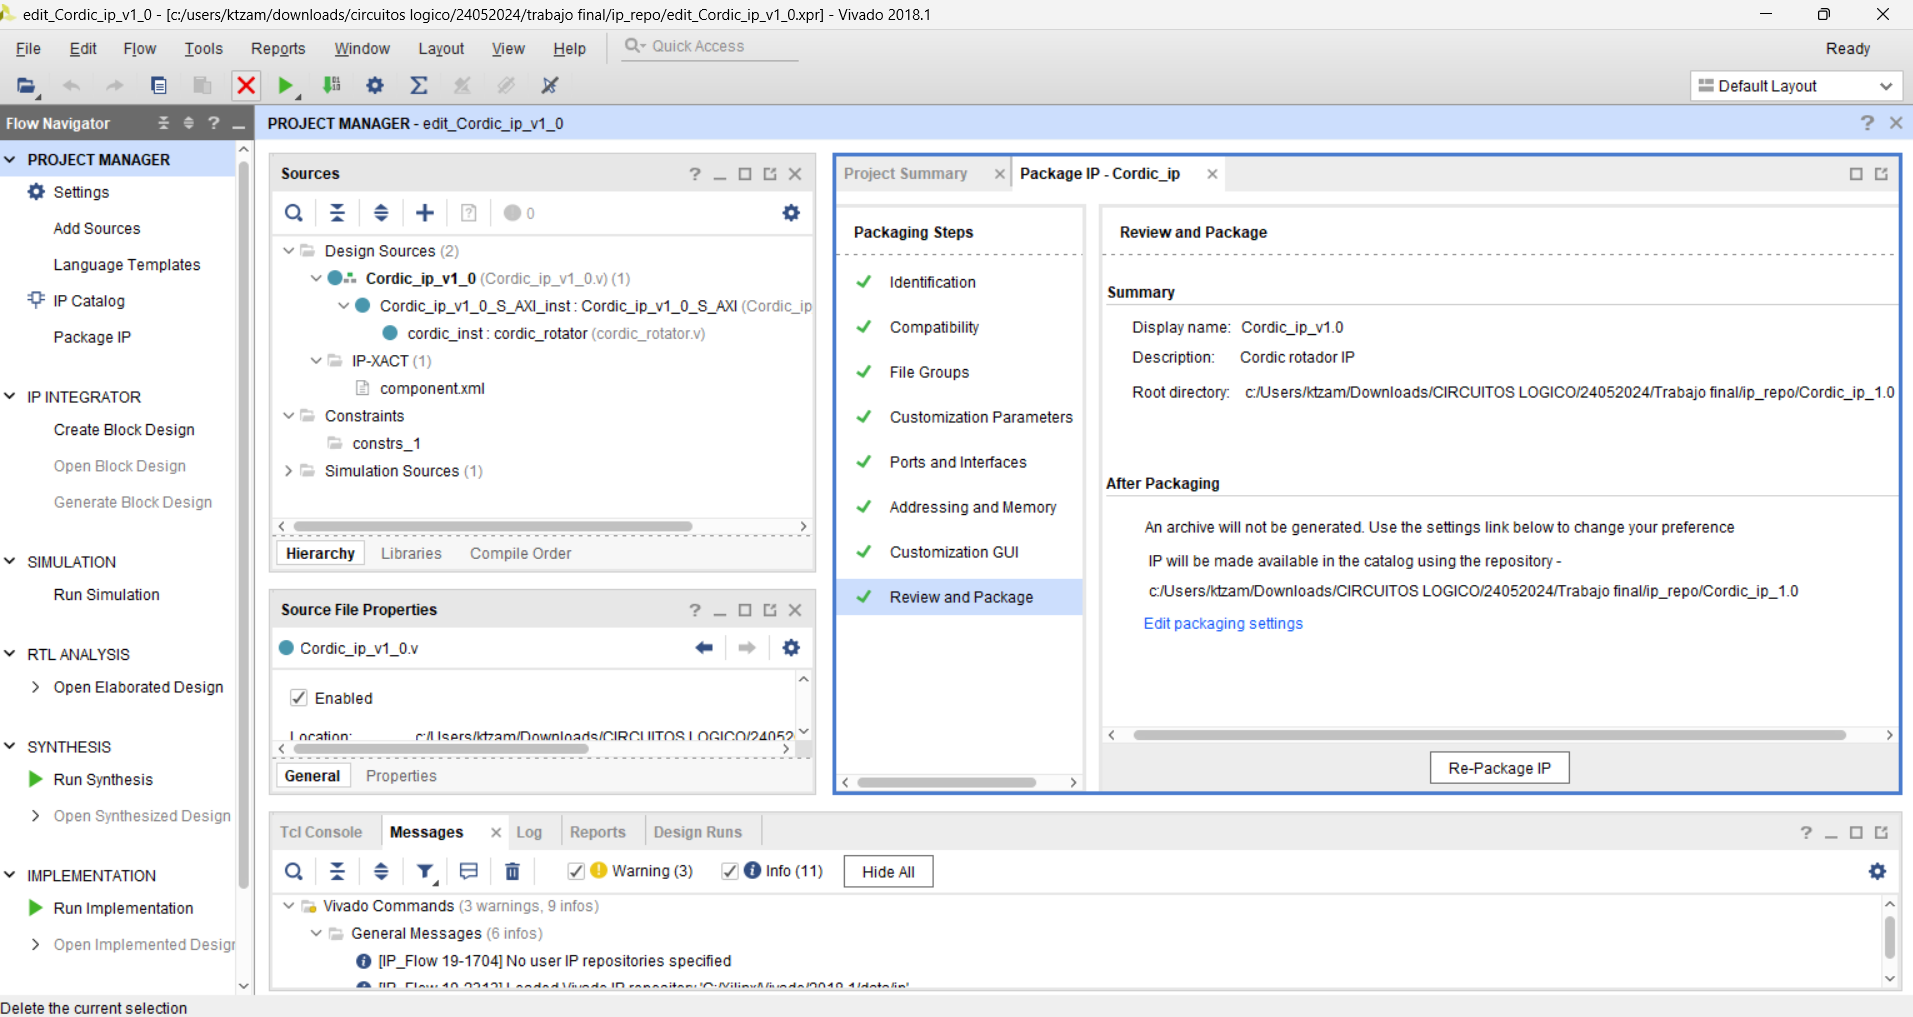
\includegraphics[width=0.8\textwidth]{./Figuras/ip_cordic.png}
\captionof{figure}{Flujo de trabajo creación IP.}
\label{fig:Flujo de trabajo creación IP}
\end{figure}

La imagen muestra el panel de control del Vivado Design Suite, una herramienta de diseño de hardware para dispositivos FPGA de Xilinx. En este panel, se muestra el flujo de trabajo para crear y empaquetar un bloque de propiedad intelectual (IP) denominado "Cordic IP\_v1\_0". Por otro lado, la compatibilidad de IP pre-producción en paquetes IP de Vivado para dispositivos Zynq es un aspecto crucial a considerar en el proceso de diseño. Los IP pre-producción son bloques de propiedad intelectual en desarrollo que aún no están completamente calificados para su implementación en diseños de producción. Xilinx puede ofrecer IP pre-producción para dispositivos Zynq como una opción para que los diseñadores comiencen a trabajar en sus proyectos antes de que el IP esté completamente finalizado. 

\begin{figure}[ht]
\centering
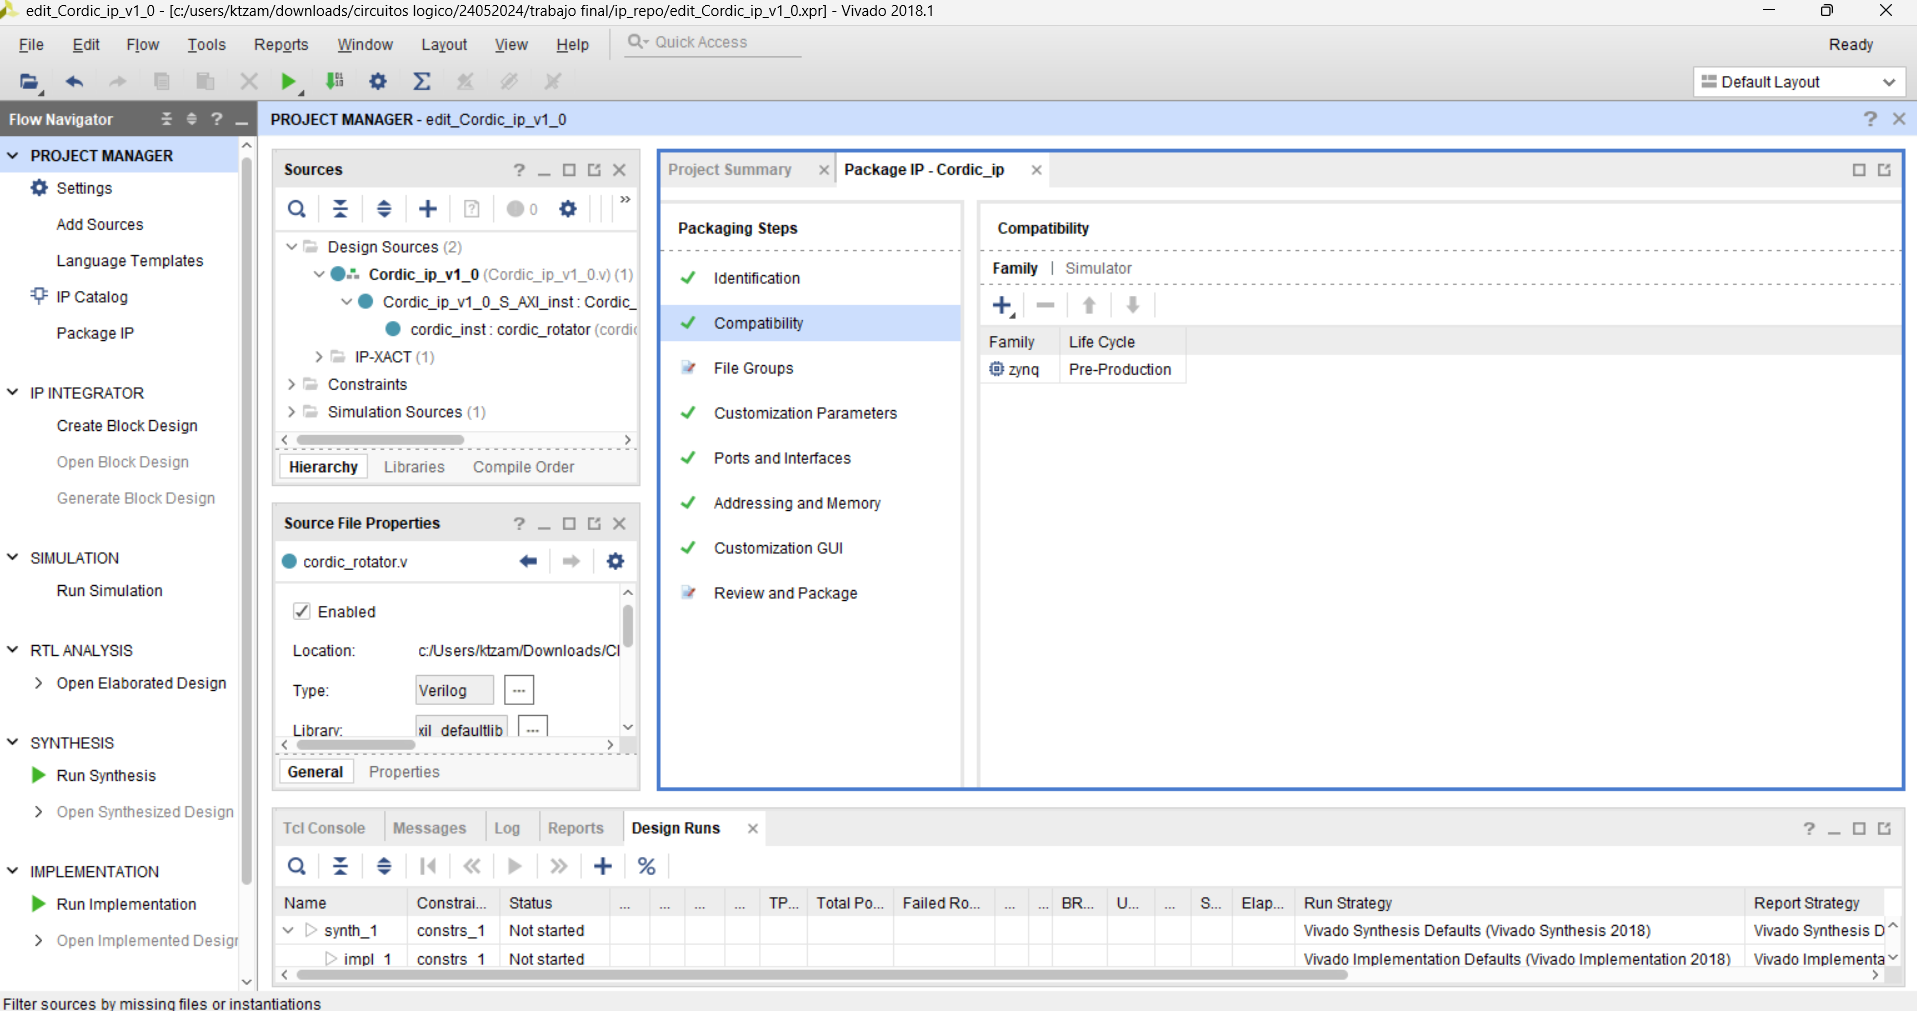
\includegraphics[width=0.8\textwidth]{./Figuras/zinq.png}
\captionof{figure}{Flujo de trabajo creación IP.}
\label{fig:Flujo de trabajo creación IP}
\end{figure}

Estos paquetes IP contienen todos los elementos necesarios para utilizar un IP en un diseño de Vivado, incluyendo el código fuente, archivos de simulación y documentación. Sin embargo, es importante tener en cuenta que los IP pre-producción pueden no ser compatibles con todas las versiones de Vivado o todos los dispositivos Zynq. Además, su uso conlleva riesgos, como la posibilidad de errores o la falta de soporte completo por parte de Xilinx. Por lo tanto, se recomienda verificar la compatibilidad del IP pre-producción con la versión de Vivado y el dispositivo Zynq específico que se está utilizando. En caso de planificar el uso del diseño en producción, es aconsejable migrar a un IP con calificación de producción tan pronto como sea posible para evitar posibles problemas y garantizar un soporte adecuado.

\newpage

\section{Inclusión de IP en el código}

En esta sección se describe el proceso de inclusión de un núcleo de propiedad intelectual (IP) personalizado en un proyecto utilizando Vivado Design Suite. Se detallan los pasos para modificar la configuración del proyecto, agregar la IP personalizada al diseño y generar el modelo top-level y exportar el diseño de hardware al SDK. La inclusión de IPs personalizadas permite reutilizar módulos de diseño ya desarrollados, facilitando y acelerando el proceso de desarrollo de sistemas complejos.


\subsection{Modificar la configuración del proyecto}

\begin{enumerate}
    \item Hacer click en Settings en el panel Flow Navigator.
    \item Seleccionar IP $\rightarrow$ Repository en el panel izquierdo de la ventana de configuración del proyecto.
    \item Hacer click en el símbolo + y navegar hasta el directorio cordic\_ip donde se estableció el repositorio. Aparecerá un mensaje indicando que se agregó un repositorio al proyecto. Presionar OK.
\end{enumerate}


\subsection{Agregar la IP personalizada}


El panel de control de Vivado Design Suite en la etapa de IP Repositories, donde se gestionan los repositorios de IP que contienen los bloques empaquetados. En el repositorio "ip\_repo", se encuentra disponible el IP Cordic\_ip\_v1.0, el cual puede ser utilizado en otros diseños dentro del mismo proyecto o en proyectos diferentes que tengan acceso al repositorio. Este enfoque facilita la reutilización de IP y promueve la eficiencia en el desarrollo de diseños complejos en Vivado Design Suite. De esta manera es neceseario implementar los siguietes pasos para agregar Cordic\_ip\_v1.0 al trabajo:

\begin{enumerate}
    \item Hacer click sobre Open Block Design debajo de IP Integrator en el panel Flow Navigator.
    \item En la ventana Diagram hacer botón derecho y seleccionar Add IP ... y buscar Cordic\_ip\_v1.0 en el catálogo colocando sum en el campo de búsqueda.
    \item Hacer doble click cobre Cordic\_ip\_v1.0 para agregarla al diseño.
\end{enumerate}

La siguiente imagen ofrece una visión del panel de control de Vivado Design Suite en la fase de IP Repositories, donde se administra la colección de repositorios de propiedad intelectual (IP)

\begin{figure}[ht]
\centering
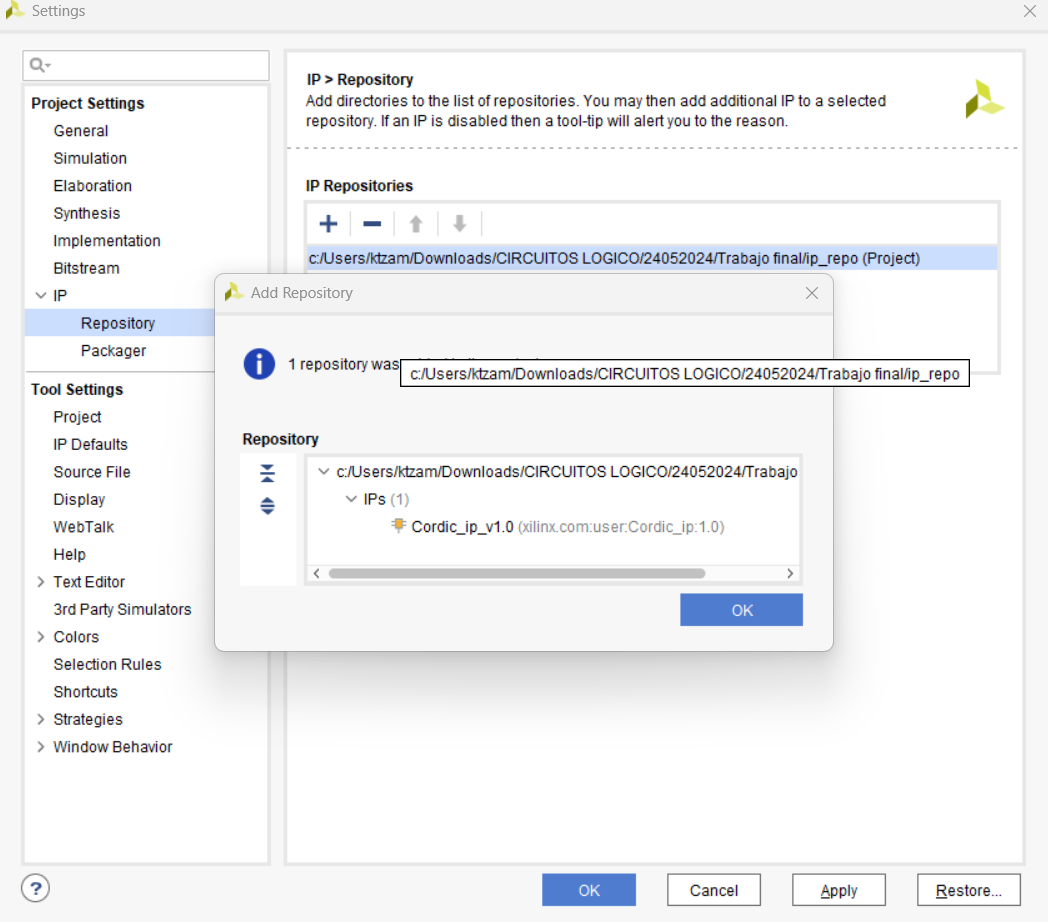
\includegraphics[width=0.7\textwidth]{./Figuras/extracción_ip.png}
\captionof{figure}{Flujo de trabajo creación IP.}
\label{fig:Flujo de trabajo creación IP}
\end{figure}


\section{Diagrama de bloques }

La imagen que me enviaste muestra un diagrama de bloques de un sistema informático basado en un System on Chip (SoC) Zynq-7000 de Xilinx, que incluye componentes principales como el Zynq-7000 Processing System, encargado de ejecutar instrucciones y realizar cálculos, y la memoria DDR3, que actúa como la memoria principal para almacenamiento temporal de datos e instrucciones.

\begin{figure}[ht]
\centering
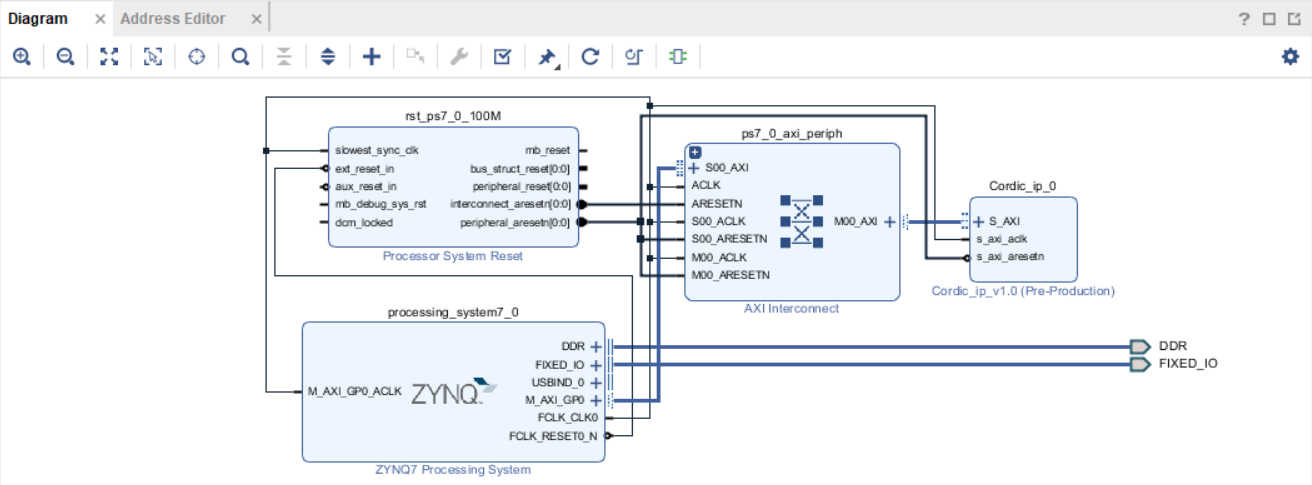
\includegraphics[width=0.8\textwidth]{./Figuras/Diagrama.png}
\captionof{figure}{Diagrama de bloques.}
\label{fig:Diagrama de bloques}
\end{figure}


\subsection{Generar el Top-Level y Export el diseño de hardware al SDK}

\begin{enumerate}
    \item En el panel Sources, hacer click-derecho sobre system.bd, y seleccionar Generate Output Products … y presionar Generate para generar los archivos de implementación, simulación y síntesis para el diseño (también puede hacer click sobre Generate Block Design en el panel Flow Navigator para hacer lo mismo).
    \item Hacer click-derecho nuevamente sobre system.bd, y seleccionar Create HDL Wrapper… para generar el modelo top-level de VHDL.
    
\end{enumerate}

\subsubsection{Generación de HDL}

En este paso, se procederá a la generación del código HDL (Hardware Description Language) a partir del diseño en bloque creado. Este código es fundamental para la implementación y síntesis del diseño en el hardware. Asegúrese de seguir cuidadosamente los pasos mencionados anteriormente para garantizar una correcta generación del código HDL.

\begin{figure}[ht]
\centering
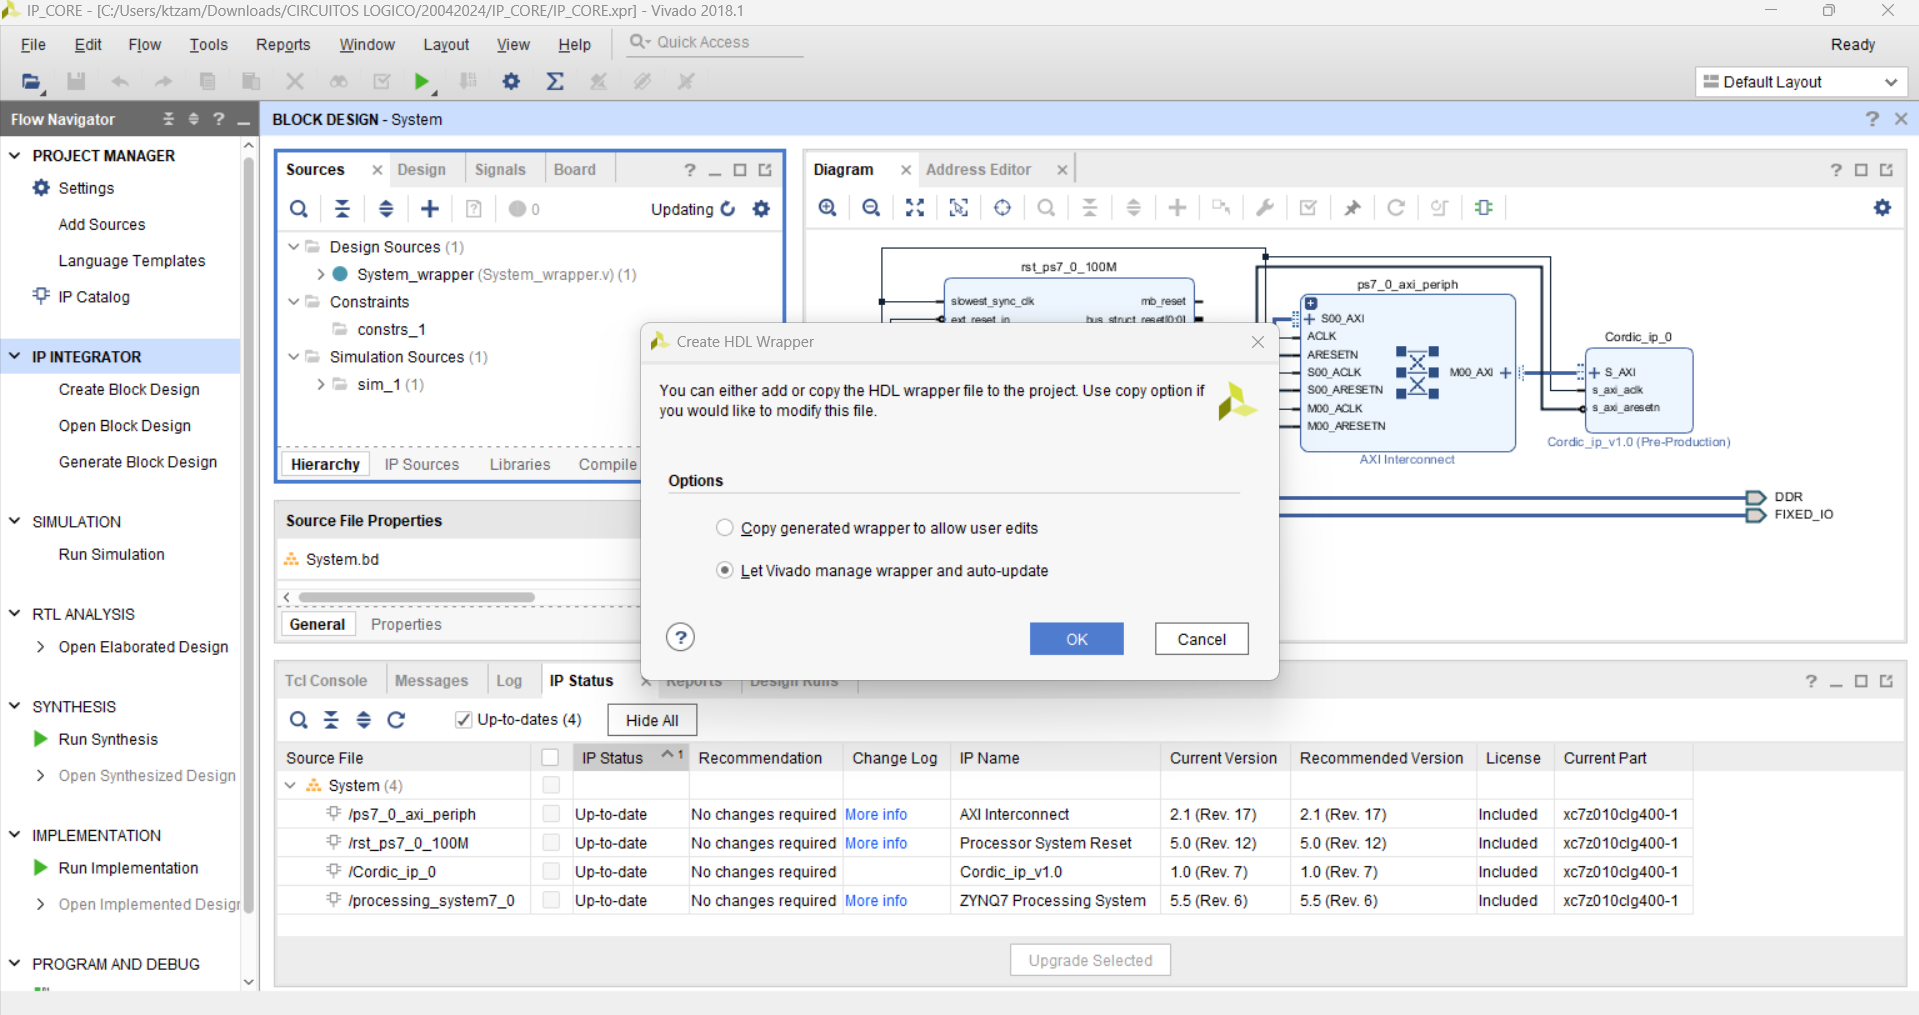
\includegraphics[width=0.8\textwidth]{./Figuras/Generar_HDL.png}
\captionof{figure}{Generar HDL.}
\label{fig:Generar HDL}
\end{figure}

\subsubsection{Exportación de hardware}

Una vez generado el código HDL, el siguiente paso es exportar el diseño de hardware. Este proceso implica preparar el diseño para su implementación en un dispositivo físico, como una FPGA. La exportación del hardware incluye la generación de archivos necesarios para la configuración y el funcionamiento del dispositivo.

\begin{figure}[ht]
\centering
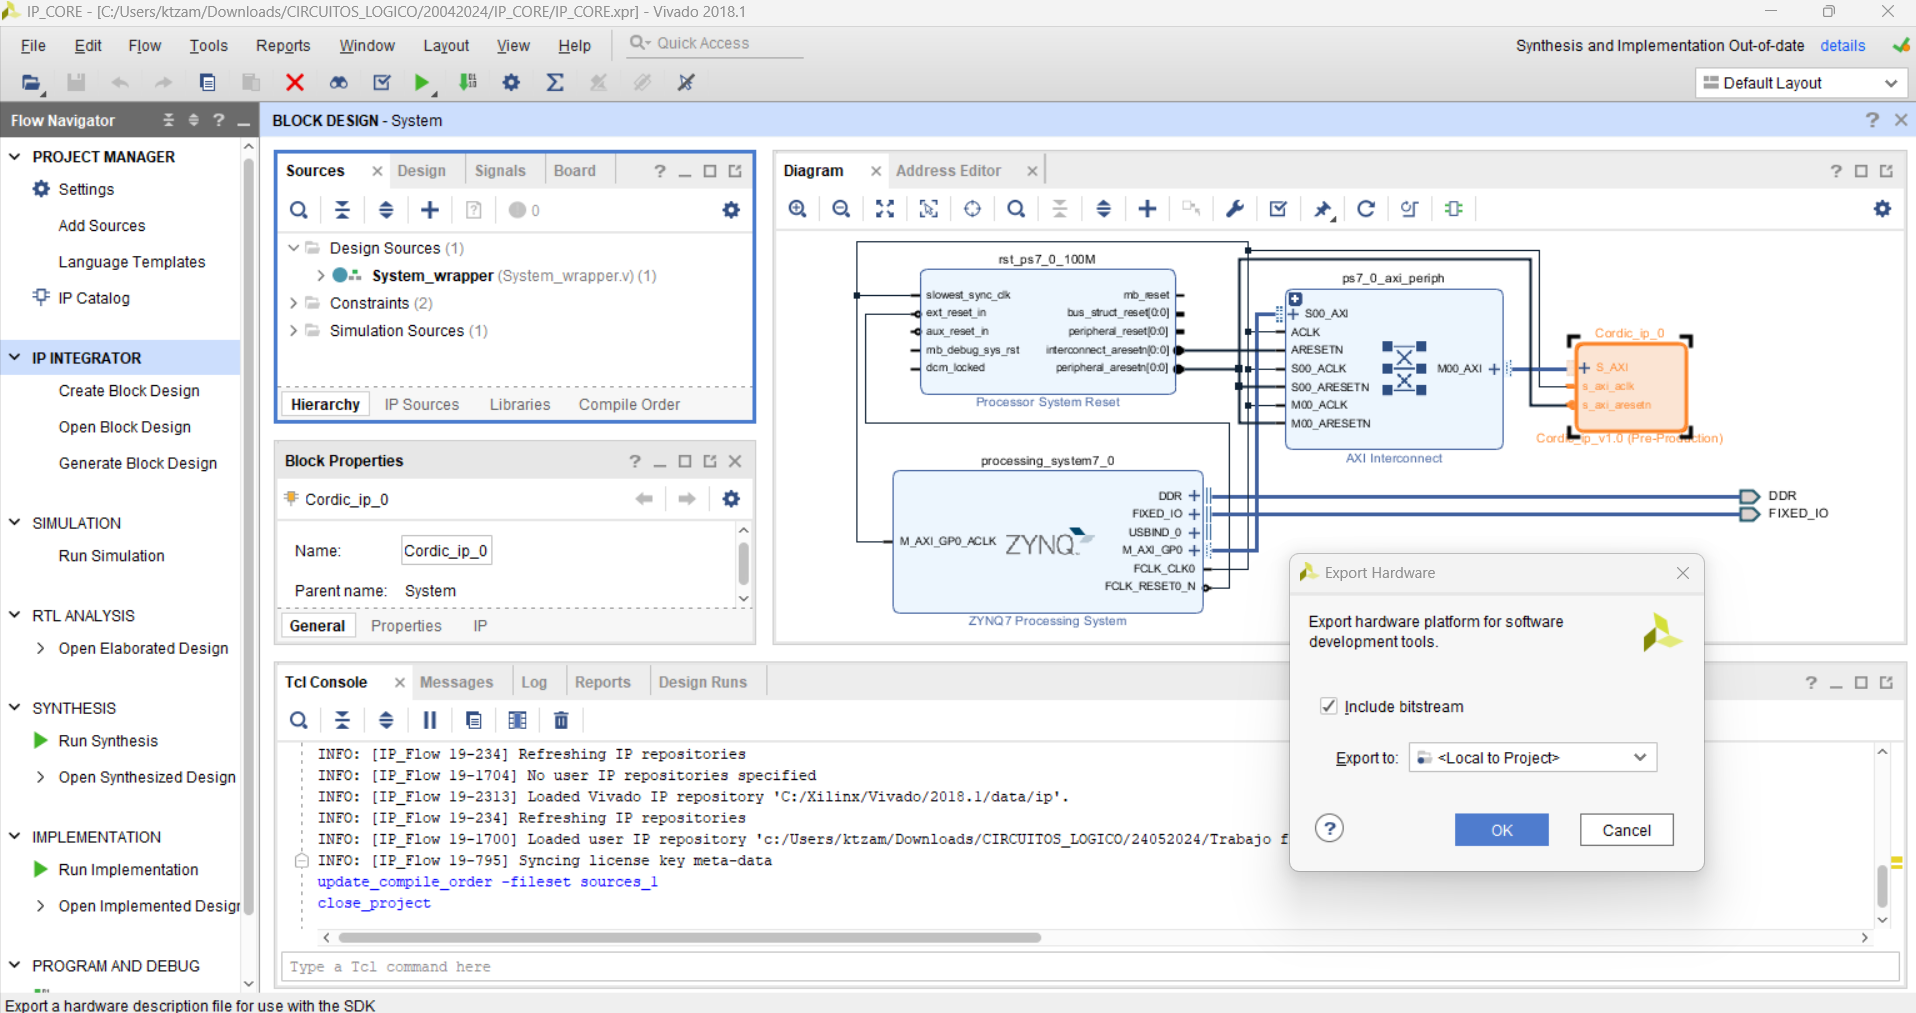
\includegraphics[width=0.8\textwidth]{./Figuras/export_hardware.png}
\captionof{figure}{Exportar hardware.}
\label{fig:Generar HDL}
\end{figure}

\subsubsection{Lanzamiento del SDK}

El SDK (Software Development Kit) es una herramienta crucial para el desarrollo de software embebido. Después de exportar el hardware, se debe lanzar el SDK para comenzar el desarrollo de software sobre el diseño de hardware implementado. Este paso asegura que el entorno de desarrollo está correctamente configurado para trabajar con el hardware.

\begin{figure}[ht]
\centering
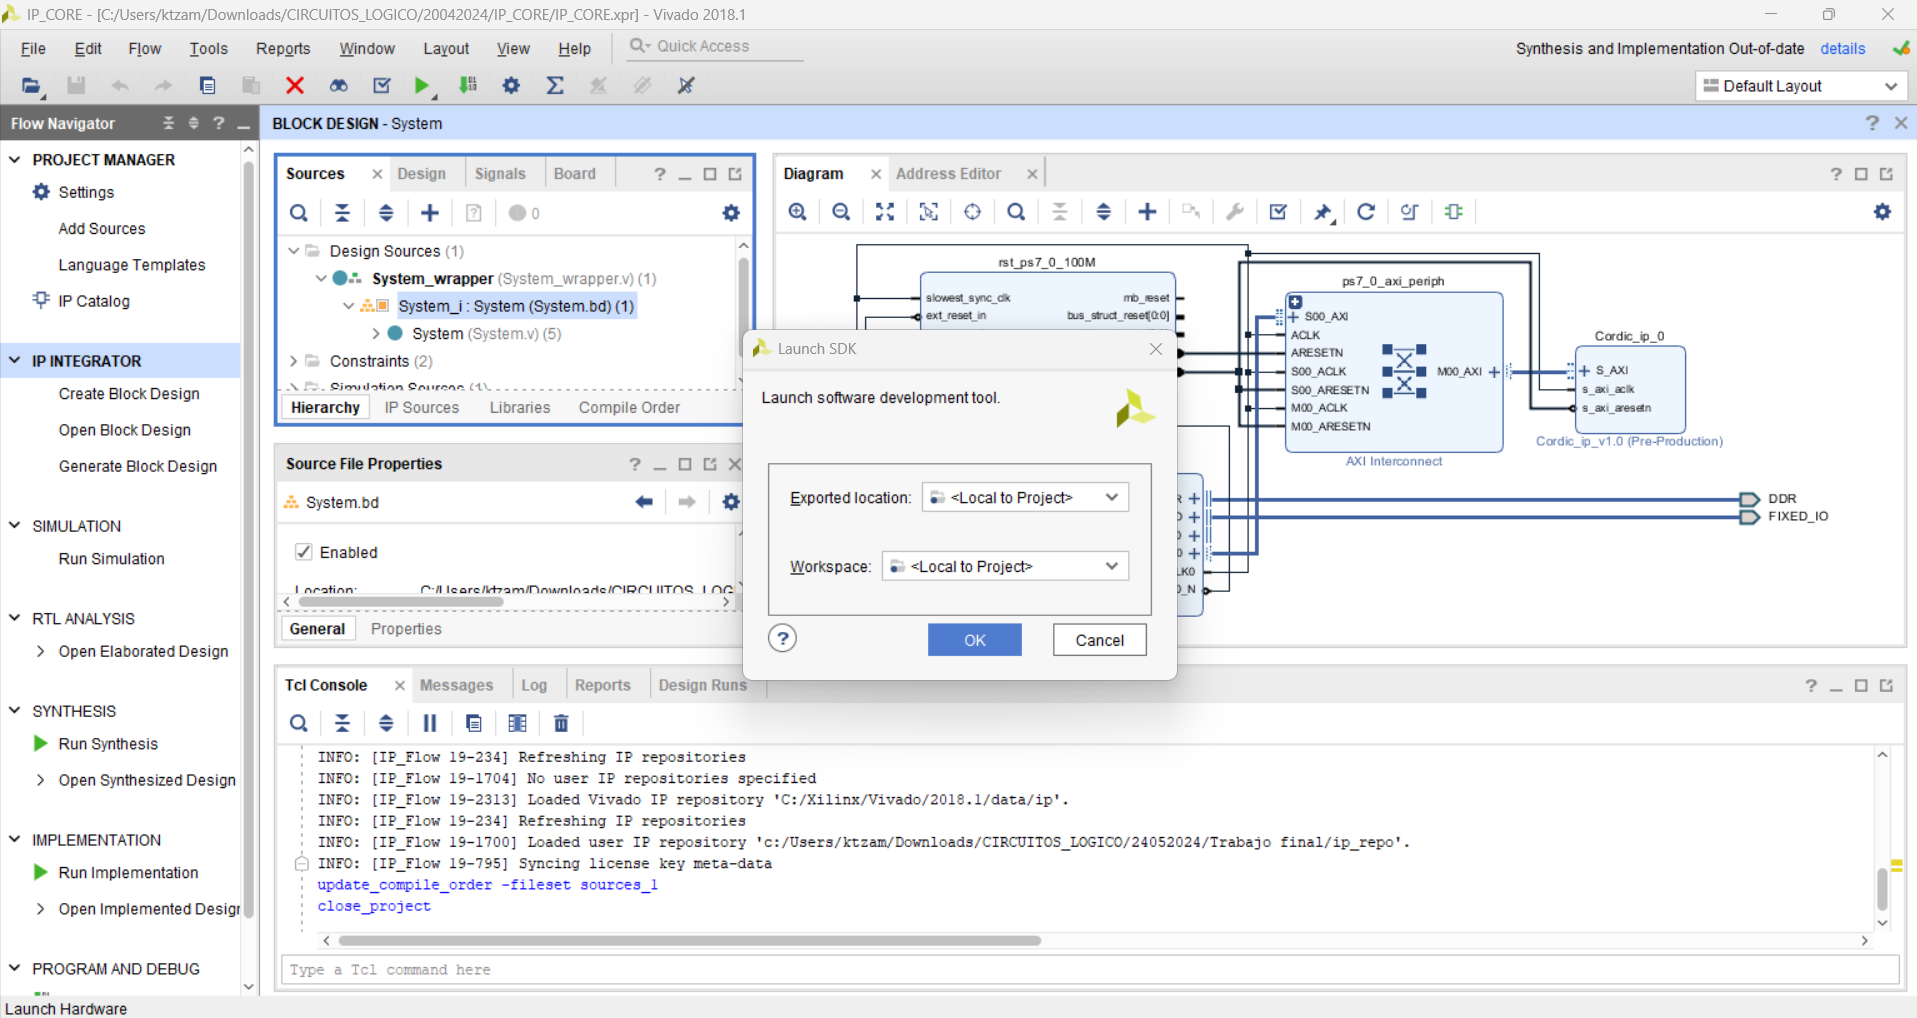
\includegraphics[width=0.8\textwidth]{./Figuras/launch_sdk.png}
\captionof{figure}{launch SDK}
\label{fig:launch SDK}
\end{figure}

\subsubsection{Creación de proyecto en Empty Application}

Dentro del SDK, se creará un nuevo proyecto utilizando la plantilla de aplicación vacía (Empty Application). Esto proporciona una base limpia y sencilla sobre la cual construir el software necesario para interactuar con el hardware exportado. Asegúrese de seleccionar la opción correcta para iniciar con un entorno de desarrollo adecuado.

\begin{figure}[ht]
\centering
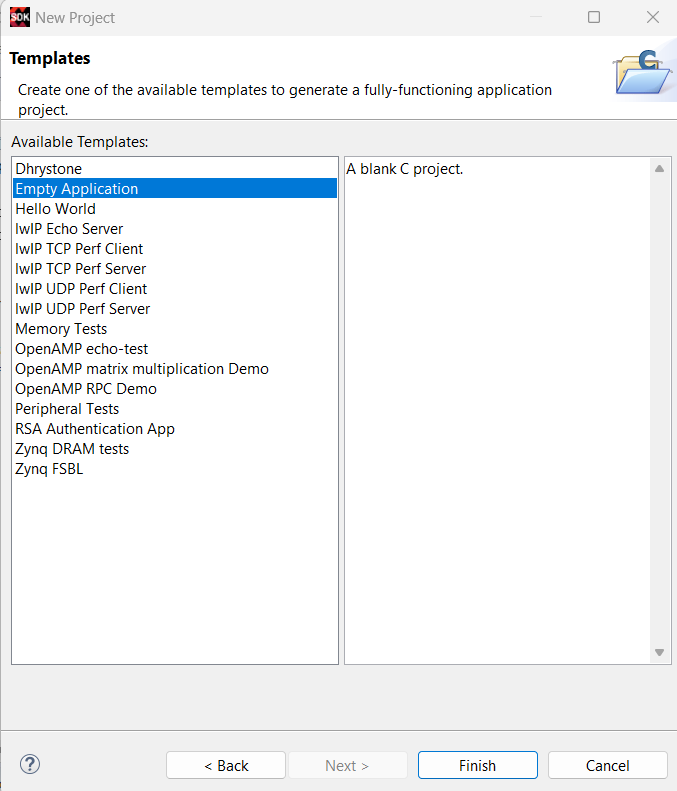
\includegraphics[width=0.6\textwidth]{./Figuras/empty_application.png}
\captionof{figure}{Empty application}
\label{fig:Empty application}
\end{figure}





\section{Conectar a servidor y validaccion de código.}

En esta sección se describe el proceso de conexión al servidor y la configuración del entorno de desarrollo de software (SDK) para programar y validar el uso de IP cores propios en una FPGA. La conexión al servidor es crucial para la comunicación y transferencia de datos entre el equipo de desarrollo y la FPGA. Posteriormente, se detalla el uso del SDK para cargar y ejecutar el código en el hardware.


\subsection{Conectar a servidor}


Se aseguró de que el servidor estuviera conectado y se configuró la terminal con una velocidad de 115200. Luego, se conectó al puerto correspondiente.

\begin{figure}[ht]
\centering
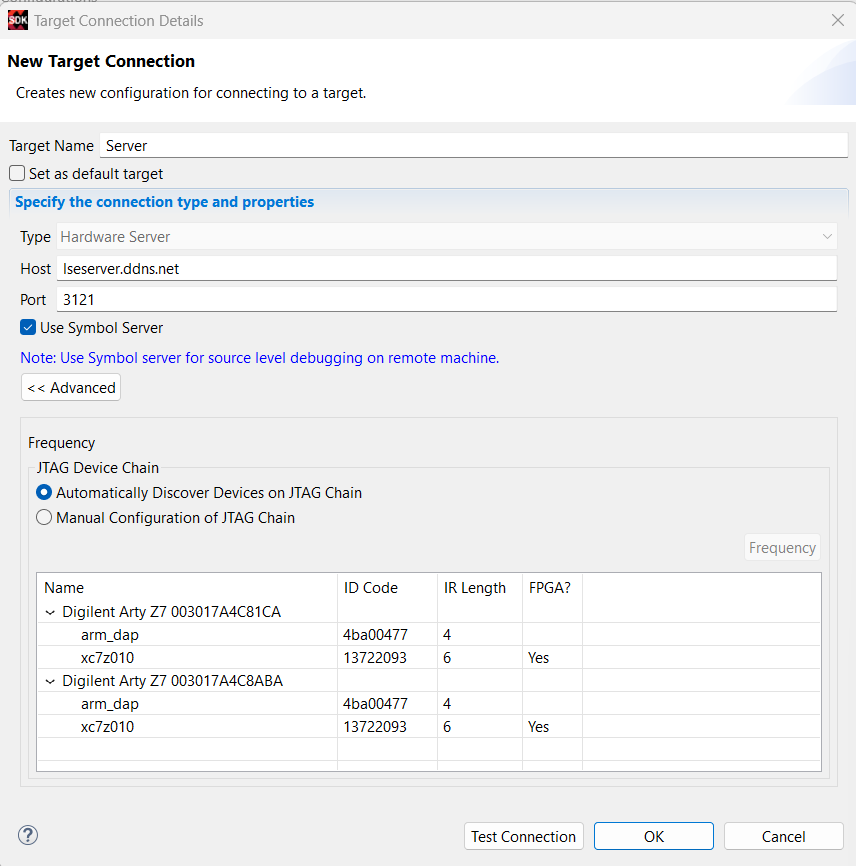
\includegraphics[width=0.8\textwidth]{./Figuras/conexion_servidor.png}
\captionof{figure}{Conexión a servidor}
\label{fig:Conexión a servidor}
\end{figure}



\subsection{Código para validar el Uso de IP cores propios}

A continuación se presenta el código en C para validar el uso de IP cores propios utilizando una IP CORDIC en un entorno FPGA. El código inicializa la IP, escribe valores de entrada, lee los valores de salida, y ejecuta una auto-prueba para verificar la funcionalidad de la IP.


\begin{figure}[ht]
\centering
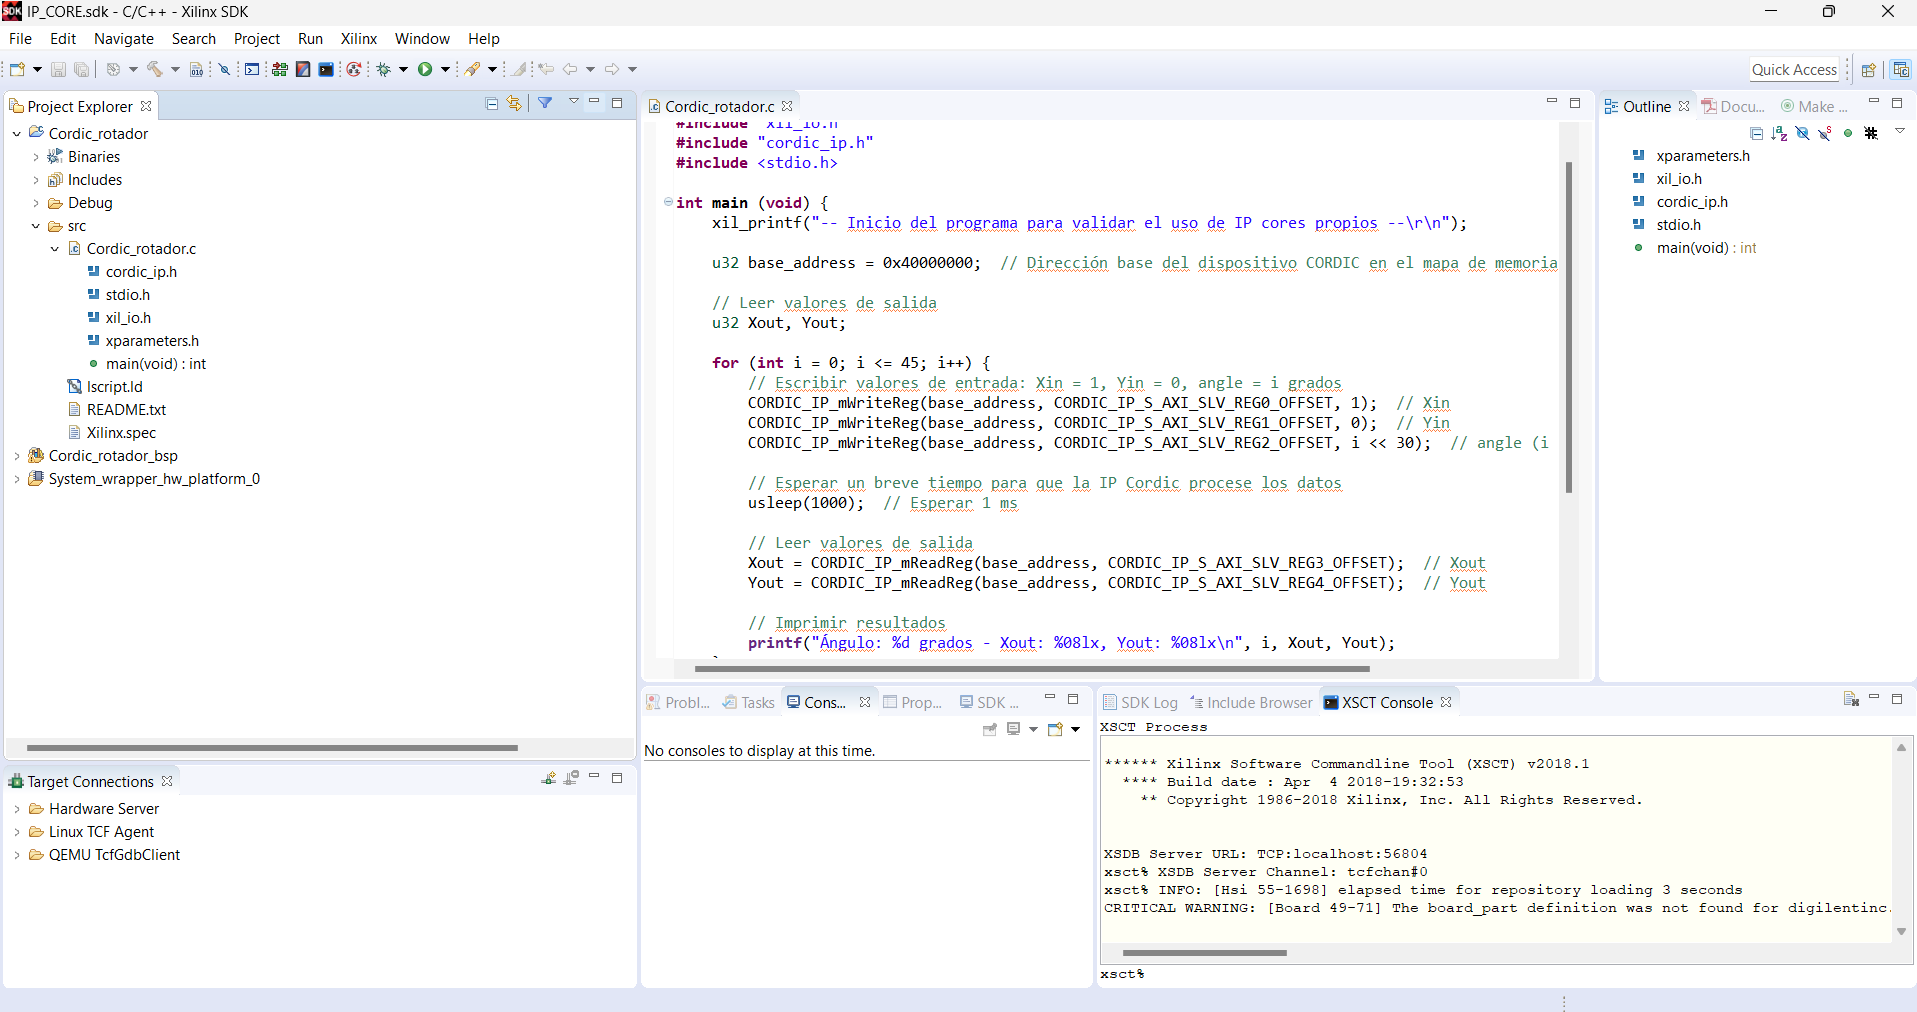
\includegraphics[width=0.8\textwidth]{./Figuras/Proyecto_SDK.png}
\captionof{figure}{SDK}
\label{fig:Visualizacion de codigo c en SDK}
\end{figure}


El código comienza incluyendo los archivos de cabecera necesarios: \texttt{xparameters.h} (proporciona las direcciones base de los dispositivos periféricos), \texttt{xil\_io.h} (define funciones de entrada/salida para el sistema), \texttt{cordic\_ip.h} (define las funciones y macros específicas para la IP CORDIC), y \texttt{stdio.h} (proporciona funciones estándar de entrada/salida en C). 

En la función \texttt{main}, se imprime un mensaje indicando el inicio del programa, se define la dirección base del dispositivo CORDIC, y se declaran las variables para almacenar los valores de salida (\texttt{Xout} y \texttt{Yout}). En un bucle de 0 a 45 grados, se escriben los valores de entrada para \texttt{Xin}, \texttt{Yin} y el ángulo, y se espera brevemente para que la IP CORDIC procese los datos. Luego, se leen los valores de salida \texttt{Xout} y \texttt{Yout} y se imprimen los resultados en la consola. Finalmente, se ejecuta una auto-prueba de la IP CORDIC. Si la auto-prueba falla, se imprime un mensaje de error y se retorna \texttt{-1}. Si la auto-prueba pasa, se imprime un mensaje de éxito y se retorna \texttt{0}.


\begin{lstlisting}[language=C, caption={Código para validar el uso de IP cores propios}, label={lst:cordic_validation}, basicstyle=\ttfamily\footnotesize, keywordstyle=\color{blue}]
#include "xparameters.h"
#include "xil_io.h"
#include "cordic_ip.h"
#include <stdio.h>

int main (void) {


    u32 base_address = 0x40000000; 

    // Leer valores de salida
    u32 Xout, Yout;

    for (int i = 0; i <= 45; i++) {
        // Escribir valores de entrada: Xin = 1, Yin = 0, angle = i grados
        CORDIC_IP_mWriteReg(base_address, CORDIC_IP_S_AXI_SLV_REG0_OFFSET, 1); 
        CORDIC_IP_mWriteReg(base_address, CORDIC_IP_S_AXI_SLV_REG1_OFFSET, 0);  
        CORDIC_IP_mWriteReg(base_address, CORDIC_IP_S_AXI_SLV_REG2_OFFSET, i << 30);

        // Esperar un breve tiempo para que la IP Cordic procese los datos
        usleep(1000);

        // Leer valores de salida
        Xout = CORDIC_IP_mReadReg(base_address, CORDIC_IP_S_AXI_SLV_REG3_OFFSET);  
        Yout = CORDIC_IP_mReadReg(base_address, CORDIC_IP_S_AXI_SLV_REG4_OFFSET);  

        // Imprimir resultados
        printf("Angulo: %d grados - Xout: %08lx, Yout: %08lx\n", i, Xout, Yout);
    }

    // Ejecutar auto-prueba
    if (CORDIC_IP_Reg_SelfTest((void *)base_address) != XST_SUCCESS) {
        printf("CORDIC IP self-test failed.\n");
        return -1;
    }

    printf("CORDIC IP self-test passed.\n");
    return 0;
}
\end{lstlisting}




\newpage

\section{Conclusiones}

En este documento, hemos abordado en detalle la implementación y validación de un módulo CORDIC Rotator en Verilog, su integración en un entorno FPGA utilizando Vivado Design Suite y su posterior verificación mediante un entorno de desarrollo de software (SDK). A continuación, se resumen los puntos clave:

\begin{enumerate}
    \item \textbf{Implementación del Módulo CORDIC Rotator:}
    \begin{itemize}
        \item Se explicó cómo se configura el módulo en Verilog, comenzando con la definición de parámetros como el ancho de bits de entrada y salida.
        \item La implementación detalló la tabla de arco tangente y las diferentes iteraciones del algoritmo CORDIC para realizar rotaciones de vectores en el plano cartesiano.
        \item Se cubrieron los ajustes necesarios para manejar ángulos de rotación en los cuatro cuadrantes del sistema cartesiano.
    \end{itemize}
    
    \item \textbf{Creación de una IP Personalizada:}
    \begin{itemize}
        \item Se describió el proceso de crear una IP personalizada en Vivado, utilizando el módulo CORDIC Rotator.
        \item El uso del template de periférico esclavo de Vivado y la configuración de los registros y parámetros necesarios para la IP.
        \item La integración del módulo CORDIC Rotator con la IP personalizada y su conexión a través de la interfaz AXI.
    \end{itemize}
    
    \item \textbf{Flujo de Trabajo en Vivado:}
    \begin{itemize}
        \item Se explicó el flujo de trabajo completo en Vivado Design Suite, desde la creación del IP hasta la generación de productos de salida y la exportación del diseño de hardware al SDK.
        \item La importancia de realizar simulaciones y análisis RTL para verificar la funcionalidad del diseño antes de la implementación en el hardware.
    \end{itemize}
    
    \item \textbf{Incorporación de la IP en el Proyecto:}
    \begin{itemize}
        \item Se detallaron los pasos para modificar la configuración del proyecto en Vivado, agregar la IP personalizada al diseño y generar el modelo top-level.
        \item La descripción del diagrama de bloques del sistema y cómo se integran los componentes principales, incluyendo la memoria DDR3 y el Zynq-7000 Processing System.
    \end{itemize}
    
    \item \textbf{Validación del Uso de IP Cores:}
    \begin{itemize}
        \item Se presentó el código en C para validar la funcionalidad de la IP CORDIC mediante la inicialización de la IP, la escritura de valores de entrada y la lectura de los valores de salida.
        \item La importancia de realizar pruebas automáticas para asegurar la correcta operación de la IP en el entorno FPGA.
    \end{itemize}
\end{enumerate}


\newpage
\section{Bibliografía}

\begin{thebibliography}{6}
\bibitem{cordic_paper}
Smith, S. W. (1971). "Cordic Trigonometry". RADC Technical Report.

\bibitem{cordic_book}
Walther, J. S. (1971). "A unified algorithm for elementary functions". AFIPS Conference Proceedings.

\bibitem{cordic_survey}
Volder, J. E. (1959). "The Cordic Trigonometric Computing Technique". IRE Transactions on Electronic Computers.

\bibitem{verilog_book}
Palnitkar, S. (2003). "Verilog HDL: A Guide to Digital Design and Synthesis". Prentice Hall.

\bibitem{verilog_reference}
IEEE Standard for SystemVerilog. (2017). IEEE Std 1800-2017.

\bibitem{fpga_cookbook}
Vohra, D. (2015). "FPGA Prototyping by Verilog Examples: Xilinx Spartan-3 Version". Wiley-IEEE Press.

\end{thebibliography}




\end{document}
